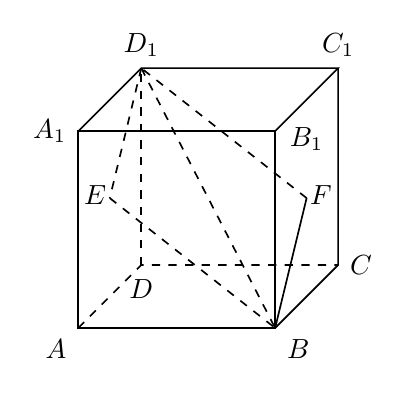
\begin{tikzpicture}[x=1cm,y=1cm,font=\normalsize,line width=.6pt]
\coordinate (A) at (0,0);
\coordinate (B) at (2.5,0);
\coordinate (B1) at (2.5,2.5);
\coordinate (A1) at (0,2.5);
\coordinate (D) at (0.8,0.8);
\coordinate (C) at (3.3,0.8);
\coordinate (C1) at (3.3,3.3);
\coordinate (D1) at (0.8,3.3);
\coordinate (E) at (0.4000000000,1.6500000000);
\coordinate (F) at (2.9000000000,1.6500000000);
% front face solid
\draw (A) -- (B) -- (B1) -- (A1) -- cycle;
% top and right visible edges
\draw (A1) -- (D1) -- (C1) -- (B1);
\draw (C1) -- (C) -- (B);
% hidden bottom edges
\draw[dashed] (A) -- (D) -- (C);
\draw[dashed] (D) -- (D1);
% quadrilateral B-F-D1-E
\draw (B) -- (F);
\draw[dashed] (F) -- (D1);
\draw[dashed] (D1) -- (E);
\draw[dashed] (E) -- (B);
% space diagonal D1-B
\draw[dashed] (D1) -- (B);
% labels clear of strokes
\node[inner sep=2pt,anchor=north east] at ([xshift=-2pt,yshift=-2pt]A) {$A$};
\node[inner sep=2pt,anchor=north west] at ([xshift=2pt,yshift=-2pt]B) {$B$};
\node[inner sep=2pt,anchor=west] at ([xshift=2pt]C) {$C$};
\node[inner sep=2pt,anchor=north] at ([yshift=-3pt]D) {$D$};
\node[inner sep=2pt,anchor=east] at ([xshift=-2pt]A1) {$A_{1}$};
\node[inner sep=2pt,anchor=west,xshift=1pt,yshift=-3pt] at ([xshift=2pt]B1) {$B_{1}$};
\node[inner sep=2pt,anchor=south] at ([yshift=2pt]C1) {$C_{1}$};
\node[inner sep=2pt,anchor=south] at ([yshift=2pt]D1) {$D_{1}$};
\node[inner sep=2pt,anchor=east,xshift=3pt,yshift=1pt] at ([xshift=-2pt]E) {$E$};
\node[inner sep=2pt,anchor=west,xshift=-3pt,yshift=1pt] at ([xshift=2pt]F) {$F$};
\end{tikzpicture}
